\newpage
\section{Протоколы обмена данными в автоматизированных системах контроля}
\setcounter{figure}{0}

На рынке представлено множество датчиков, которые связываются с системой по различным протоколам. Используются такие протоколы как \cite{csp}:
\begin{itemize}
\item TCP/IP;
\item Modbus;
\item Canbus;
\item МЭК 60870-5-101;
\item МЭК 60870-5-104;
\item ОРС;
\item "Пирамида" (закрытый протокол);
\item спецпротоколы электросчетчиков;
\item SNMP;
\item TFTP;
\item RTU-325.
\end{itemize}

\subsection{Стандарт OPC}

OPC (OLE for Process Control) – семейство протоколов, предоставляющих единый интерфейс для управления объектами автоматизации и технологическими процессами. В частности, OPC DA (DataAccess) — стандарт, описывающий набор функций обмена данными в реальном времени с объектами автоматизации. 

Спецификация OPC охватывает:
\begin{itemize}
 \item концепцию клиент-серверную технологию OPC и определение данных;
 \item описания интерфейсов, методов, параметров и возможное их поведение;
 \item описание типов и структур данных;
 \item общие виды деятельности, которые включают в себя определение адресного пространства и его просмотра. Чтение, запись и подписка на уведомления об обновлении данных.
\end{itemize}

К недостаткам этого OPC можно отнести:
\begin{itemize}
 \item необходимость платного членства в сообществе The InteroperabilityStandard for Industrial Automation;
 \item протокол основан на технологиях windows.
\end{itemize}

Данный протокол не подходит, так как для его использования необходимо платное членство, что является неприемлемым для заказчика.

\subsection{Стандарт МЭК-60870-5-101/104}

МЭК-60870-5-101/104 – это протокол передачи данных, применяется в АСКТУ, АСКУЭ. Особенности реализации протокола МЭК 60870-101/104 при передаче данных между объектом и диспетчерским центром:

\begin{itemize}
 \item передача ограниченного количества информации, что обусловлено необходимостью переназначения всех сигналов с одного протокола на другой, и, как следствие, потеря некоторых данных, передача которых на этапе проектирования не была сочтена целесообразной;
 \item отсутствие единых наименований сигналов в рамках объекта и в центрах управления сетями, приводящее к сложности наладки и отслеживания ошибок;
 \item протокол МЭК 60870-5-101 предназначен для передачи данных по последовательным линиям связи RS-232/485;
 \item протокол МЭК 60870-5-104 является расширением протокола 101 и регламентирует использование сетевого доступа по протоколу TCP/IP.
\end{itemize}

Недостатки реализации данного стандарта:

\begin{itemize}
 \item количество передаваемых сигналов ограничивается определенным количеством дискретных входов и выходов;
 \item отсутствует возможность контроля связи между устройствами;
 \item возможно ложное срабатывание дискретного входа устройства при замыкании на землю в цепи передачи сигнала;
 \item цепи подвержены воздействию электромагнитных помех;
 \item сложность расширения систем;
 \item передача данных осуществляется в два этапа:
 \begin{enumerate}
  \item назначение индексированных коммуникационных объектов на прикладные объекты;
  \item  назначение прикладных объектов на переменные в прикладной базе данных или программе. Таким образом, отсутствует семантическая связь (полностью или частично) между передаваемыми данными и объектами данных прикладных функций.
 \end{enumerate}
 \item протоколы не предусматривают возможность передачи сигналов реального времени.
\end{itemize}

Данный протокол не подходит ввиду ограниченности возможностей и сложности масштабирования системы.

\subsection{Стандарт MODBUS}

Modbus – один из наиболее распространенных сетевых протоколов для интеграции устройств РЗА (релейная защита автоматики) в систему АСТУ, построенный на архитектуре «клиент–сервер». Данный протокол является открытым, что частично обуславливает его популярность. Протокол Modbus для передачи данных использует такие линиям связи как RS-485, RS-433, RS-232, а также сети TCP/IP (Modbus TCP).

Стандарт Modbus содержит в себе:

\begin{itemize}
 \item спецификация прикладного уровня;
 \item спецификация канального уровня;
 \item спецификация физического уровня;
 \item спецификацию ADU для транспорта через стек TCP/IP.
\end{itemize}

К достоинствам стандарта относится:

\begin{itemize}
 \item массовость;
 \item относительная простота реализации систем на его базе.
\end{itemize}

К недостаткам данного протокола можно отнести:

\begin{itemize}
 \item в случае необходимости отсутствует возможность оперативной сигнализации от конечного устройства к мастеру;
 \item стандарт не регламентирует начальную инициализацию системы. Назначение сетевых адресов и параметров системы для каждого устройства выполняются вручную на этапе адаптации;
 \item отсутствие  возможности  конечным  устройствам  обмениваться фиксированными данными друг с другом без участия мастера. Что ограничивает  применимость MODBUS-решений в системах регулирования реального времени.
\end{itemize}

Данный протокол не подходит ввиду отсутствия возможности оперативной сигнализации от конечного устройства к мастеру.

\subsection{Стандарт CAN}

CAN (Controller Area Network) – стандарт промышленной сети, использующийся для объединения в единую сеть устройств и датчиков. Применяется в системах автоматизации промышленного производства. 

В первую очередь данный стандарт описывает физический уровень, наибольшую популярность получил вариант описанный в ISO 11898-2. Физический уровень использует дифференциальную передачу данных по витой паре, для управления доступом к шине используется неразрушающее bit-wise разрешение конфликтов ISO 11898.

К положительным аспектам данной реализации относиться:

\begin{itemize}
 \item работа в режиме жёсткого реального времени;
 \item высокая устойчивость к помехам;
 \item надёжный контроль ошибок приема-передачи данных.
\end{itemize}

К достоинствам данного стандарта относятся:

\begin{itemize}
 \item сообщения имеют малые размеры (8 байт данных) и защищены контрольной суммой;
 \item большой размер служебных данных в пакете по отношению к полезным данным;
 \item отсутствие единого общепринятого стандарта на протокол высокого уровня (в том числе TCP).
\end{itemize}

Данный протокол не подходит из-за сложностей использования в сетях интернет.

\subsection{Стандарт DLMS}

DLMS (Device Language Message Specification) – стек протоколов, ориентированный на 16-разрядные микроконтроллеры Microchip PIC. Является международным стандартом для систем сбора данных с электро-, газовых, водяных и тепловых счетчиков. Работает на основе протоколов связи (RS232, RS485, PSTN, GSM, GPRS, IPv4, PPP и PLC), с поддержкой шифрования AES128.

Особенности данного протокола:

\begin{itemize}
 \item работает на всех 16-битных микроконтроллерах PIC и dsPIC;
 \item возможность интеграции стека DLMS с текущими реализациями протоколов TCP/IP, ZigBee и PLC;
 \item небольшой объем занимаемой памяти позволяет использовать компактные и недорогие контроллеры;
 \item для европейского рынка стек поддерживает IEC 62056-21 Mode E.
\end{itemize}

К недостаткам данного протокола можно отнести то, что описание протокола предоставляется на платной основе или требуется членство в ассоциации DLMS. Что является неприемлемым для заказчика.

Из представленного краткого анализа видно, что существующие протоколы связи достаточно успешно позволяют реализовывать задачи диспетчерского управления / интеграции данных в системы управления, однако не все они позволяют реализовывать функции реального времени. К тому же большое количество проприетарных протоколов приводит к усложнению процесса интеграции устройств в единую систему: 

\begin{itemize}
 \item протоколы должны поддерживаться контроллером, что требует реализации поддержки большого количества протоколов в в нем и ведет к удорожанию оборудования;
 \item для интеграции устройств по проприетарным протоколам требуется квалификация наладочного персонала в работе с каждым из них;
 \item переназначение сигналов из проприетарных протоколов в общепромышленные и назад часто приводит к потере информации, включая дополнительную информацию;
 \item при передаче данных по-прежнему применяется большое количество последовательных интерфейсов, что накладывает ограничения на скорость передачи данных, объем передаваемых данных и количество устройств, одновременно включенных в информационную сеть.
\end{itemize}

\subsection{Предлагаемое решение}

Большинство приборов учета (или УСПД) поддерживают протокол передачи данных TCP/IP, в виду чего использование данного протокола на транспортном уровне является целесообразным, так как в отличие от других протоколов передачи данных TCP/IP имеет следующие преимущества:

\begin{itemize}
 \item скорость разработки и цена разработки;
 \item использование в сетях интернет;
 \item более простой (простая поддержка);
 \item обеспечивает контроль целостности передаваемых данных;
 \item возможность обеспечить программную поддержку новых устройств через модульную систему драйверов.
\end{itemize}

TCP (англ. Transmission Control Protocol, протокол управления передачей) — один из основных протоколов передачи данных Интернета, предназначенный для управления передачей данных в сетях и подсетях TCP/IP\cite{tcp}.

Для обеспечения защищенного соединения необходимо использовать технологии построения виртуальных каналов. 

Технология построения защищенного соединения в открытых сетях так же позволит решить проблему конфиденциальности передаваемых данных благодаря тому, что весь передаваемый трафик передается в шифрованном виде. Примером таких технологий является технология VPN. VPN (англ. Virtual Private Network — виртуальная частная сеть\cite{vpn}) — обобщённое название технологий, позволяющих обеспечить одно или несколько сетевых соединений (логическую сеть) поверх другой сети (например, Интернет). Несмотря на то, что коммуникации осуществляются по сетям с меньшим или неизвестным уровнем доверия (например, по публичным сетям), уровень доверия к построенной логической сети не зависит от уровня доверия к базовым сетям благодаря использованию средств криптографии (шифрования, аутентификации, инфраструктуры открытых ключей, средств для защиты от повторов и изменений передаваемых по логической сети сообщений).

Так же для решения данной задачи возможно использование технологии SSH. SSH (англ. Secure Shell — «безопасная оболочка»\cite{ssh}) — сетевой протокол прикладного уровня, позволяющий производить удалённое управление операционной системой и туннелирование TCP-соединений (например, для передачи файлов). Схож по функциональности с протоколами Telnet и rlogin, но, в отличие от них, шифрует весь трафик, включая и передаваемые пароли. SSH допускает выбор различных алгоритмов шифрования. SSH-клиенты и SSH-серверы доступны для большинства сетевых операционных систем. 

Тогда последовательность действий при запросе данных от ССД к УСПД имеет следующий вид:

\begin{enumerate}
 \item установление соединения между ССД и УСПД;
 \item отправка идентификационных данных ССД на УСПД;
 \item отправка запроса на получение данных от УСПД;
 \item получение данных от УСПД;
 \item завершение соединения.
\end{enumerate}

Функциональная схема данного процесса представлена на рисунке \ref{img:get_data_idef0}.

\begin{figure}[!ht]
 \center{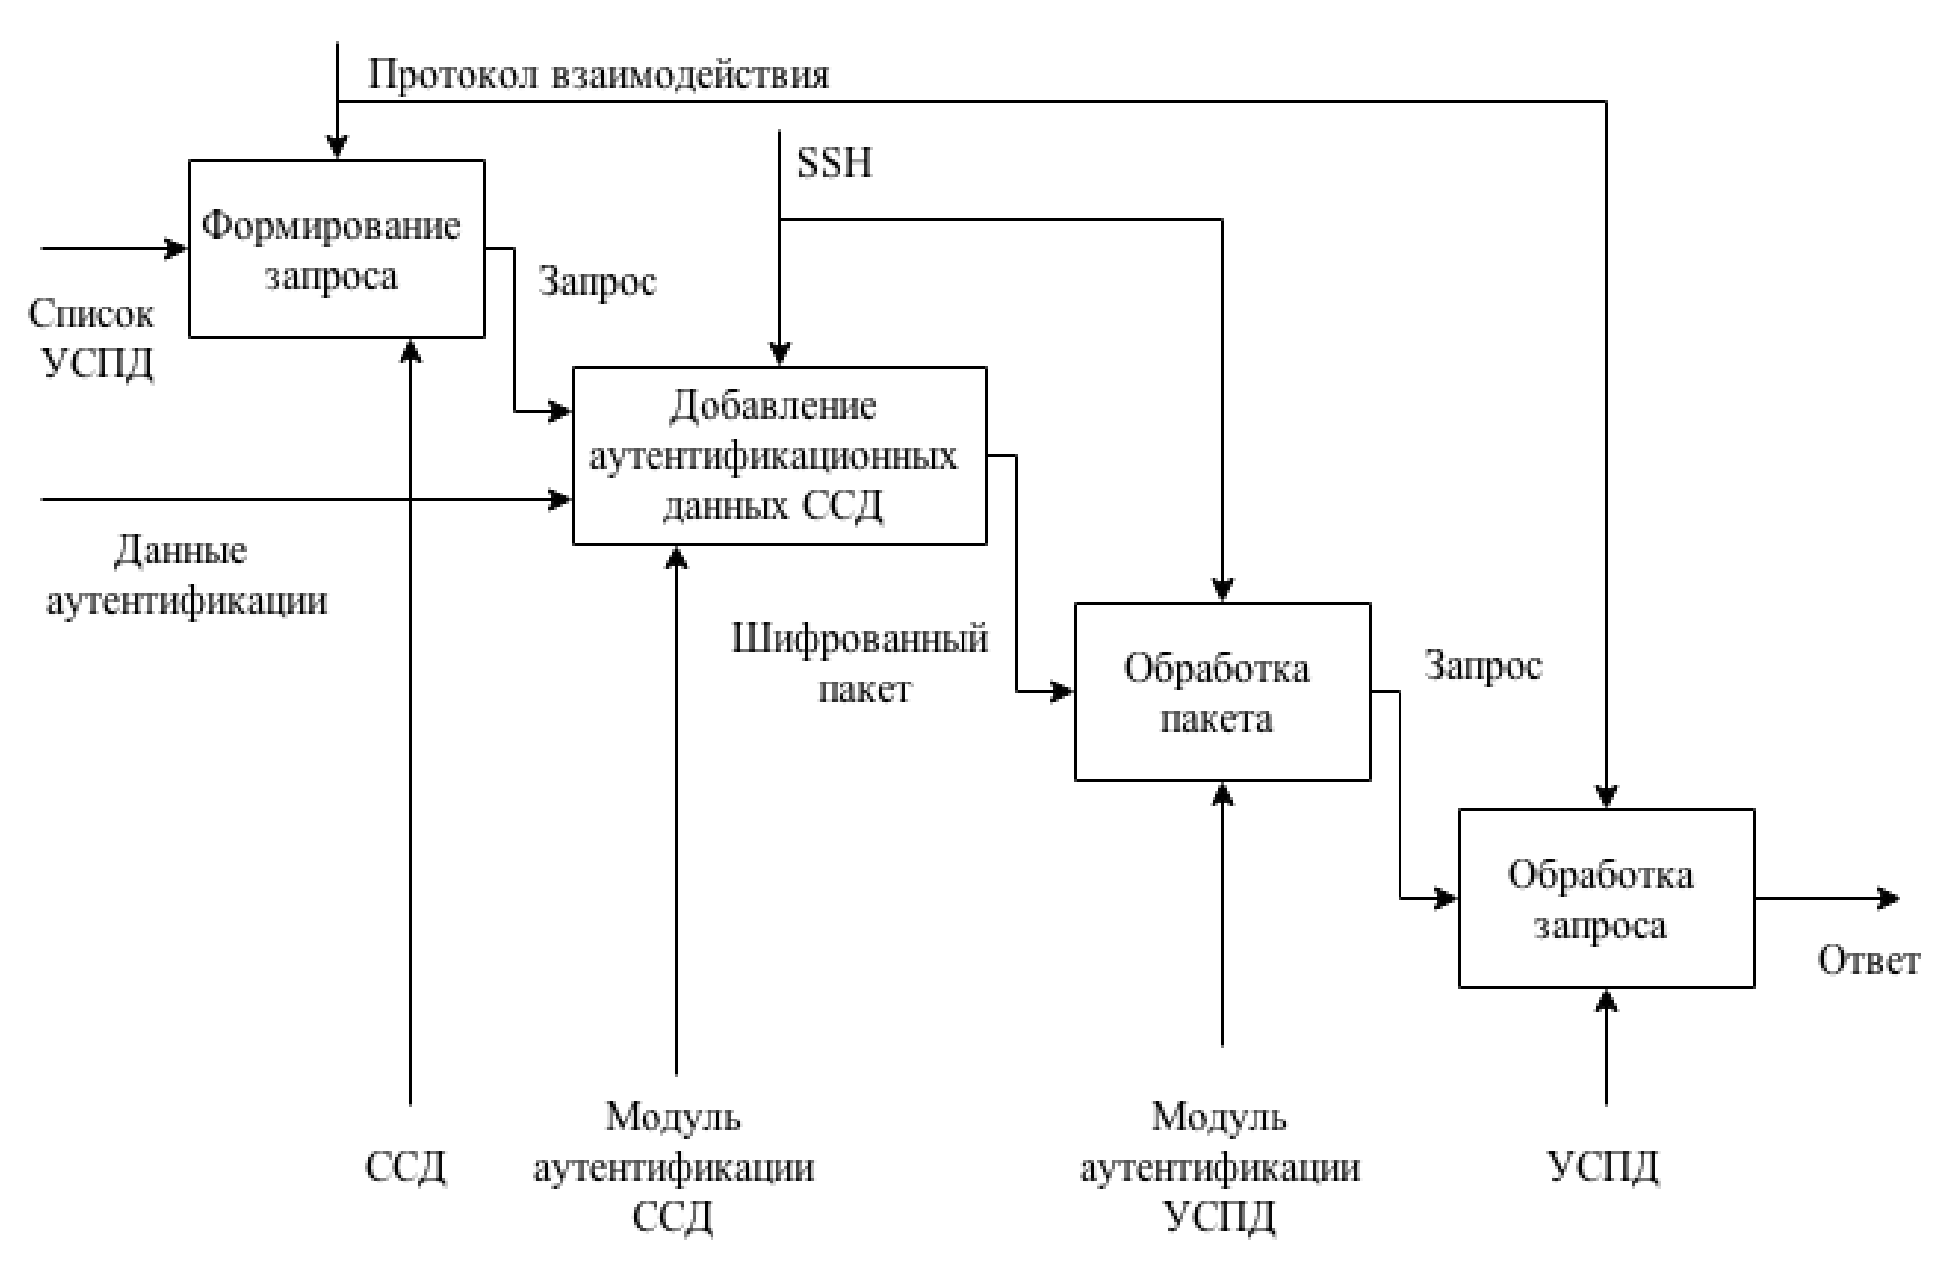
\includegraphics[width=0.8\linewidth]{get_data_idef0}}
 \caption{Запрос данных с УСПД}
 \label{img:get_data_idef0}
\end{figure}

Использование технологий построения виртуальных частных каналов позволяет защититься от угроз:

\begin{itemize}
 \item внедрение ложного объекта сети;
 \item анализ сетевого трафика;
 \item подмена доверенного объекта;
 \item навязывание ложного маршрута;
 \item выведывание паролей.
\end{itemize}

При использовании ssh в качестве средства построения защищенного канала угрозы внедрения ложного объекта закрывается, так как на всех доверенных устройствах будут находиться секретные ключи ssh, уникальный для каждого устройства. Анализ трафика так же не приносит результатов из-за шифрования. Подмена доверенного объекта исключена из-за проверки секретного ключа операционных систем. Данный ключ генерируется при установки операционной системы и проверяется при каждом подключении по ssh. Если при подключении выявляется изменение ключа, то соединение не устанавливается и появляется предупреждение. Навязывание ложного маршрута является бессмысленным ввиду шифрования трафика, как и выведывание паролей.